\documentclass[10pt, compress,usetitleprogressbar,aspectratio=1610, notes]{beamer}
% Si se quita "Notes" aparece sólo la presentación, sin notas.

\usepackage[spanish]{babel}
\usepackage{tikz}


\usetheme{epstfg}
\setbeamertemplate{note page}[compress]

\title{\LaTeX\ Crash Course}
\author{Guillermo Julián Moreno \and Pedro Valero Mejía}
\date{\today}

\begin{document}

\maketitle

\section{¿Qué es \LaTeX?}

\begin{frame}
\frametitle{¿Qué es?}

Es un \textit{document typesetting system} o, en otras palabras, un sistema para escribir documentos (y en realidad más cosas, como esta presentación).

\begin{minipage}{0.5\textwidth}
Puntos fuertes:

\begin{enumerate}
\item No hay que preocuparse (demasiado) del formato.
\item Muy potente para escribir matemáticas.
\item Paquetes extra para hacer dibujos complejos, gráficas, algoritmos...
\item ¡Se puede programar!
\end{enumerate}
\end{minipage}
\begin{minipage}{0.4\textwidth}
\begin{flushright}
\begin{tikzpicture}[scale=0.9]
  \shade[top color=blue,bottom color=gray!50]
      (0,0) parabola (1.5,2.25) |- (0,0);
  \draw (2.3cm,0.8) node[align = left]
      {$\displaystyle\int\limits_0^{3/2} \!\!x^2\mathrm{d}x$};

  \draw[style=help lines] (0,0) grid (3.9,3.9)
       [step=0.25cm]      (1,2) grid +(1,1);

  \draw[->] (-0.2,0) -- (4,0) node[right] {$x$};
  \draw[->] (0,-0.2) -- (0,4) node[above] {$f(x)$};

  \foreach \x/\xtext in {1/1, 2/2, 3/3}
    \draw[shift={(\x,0)}] (0pt,2pt) -- (0pt,-2pt) node[below] {$\xtext$};

  \foreach \y/\ytext in {1/1, 2/2, 3/3}
    \draw[shift={(0,\y)}] (2pt,0pt) -- (-2pt,0pt) node[left] {$\ytext$};

  \draw (-.5,.25) parabola bend (0,0) (2,4) node[below right] {$x^2$};
\end{tikzpicture}
\end{flushright}
\end{minipage}

\note{
\begin{enumerate}
\item \LaTeX\ sabe perfectamente cómo colocar imágenes, alinear párrafos, poner títulos y más. Nosotros sólo decimos qué queremos hacer, y el sistema hace el resto. Incluso tenemos referencias automáticas, \LaTeX\ las formatea él sólo.
\item Otros editores de texto pueden poner ecuaciones matemáticas, pero las cosas se complican cuando queremos poner alguna alineada, o matrices, o... \LaTeX\ permite hacer todo eso y más.
\item Por ejemplo, la gráfica de la derecha está hecha con código \LaTeX, no hace falta cambiar de programa.
\item Se pueden desarrollar comandos propios, escribir nuestras propias ``plantillas'' de documento, y en definitiva hacer casi cualquier cosa.
\end{enumerate}

Aquí habría que comentar que esto lo hace muy buena elección para escribir documentos matemáticos, hacer prácticas (puedes tener plantillas ya hechas, y además no es difícil hacer un script que saque cosas en \LaTeX), o incluso tomar apuntes si (como nosotros) tienes los comandos para poder escribir rápido.
}

\end{frame}

\begin{frame}
\frametitle{¿Cómo funciona?}

\LaTeX\ no es un programa como Word, es más un lenguaje de programación. Nosotros escribimos un código, entremezclando comandos y texto, y luego lo compilamos para generar un PDF.

\begin{figure}[b]
\centering
\begin{minipage}{0.48\textwidth}
\centering
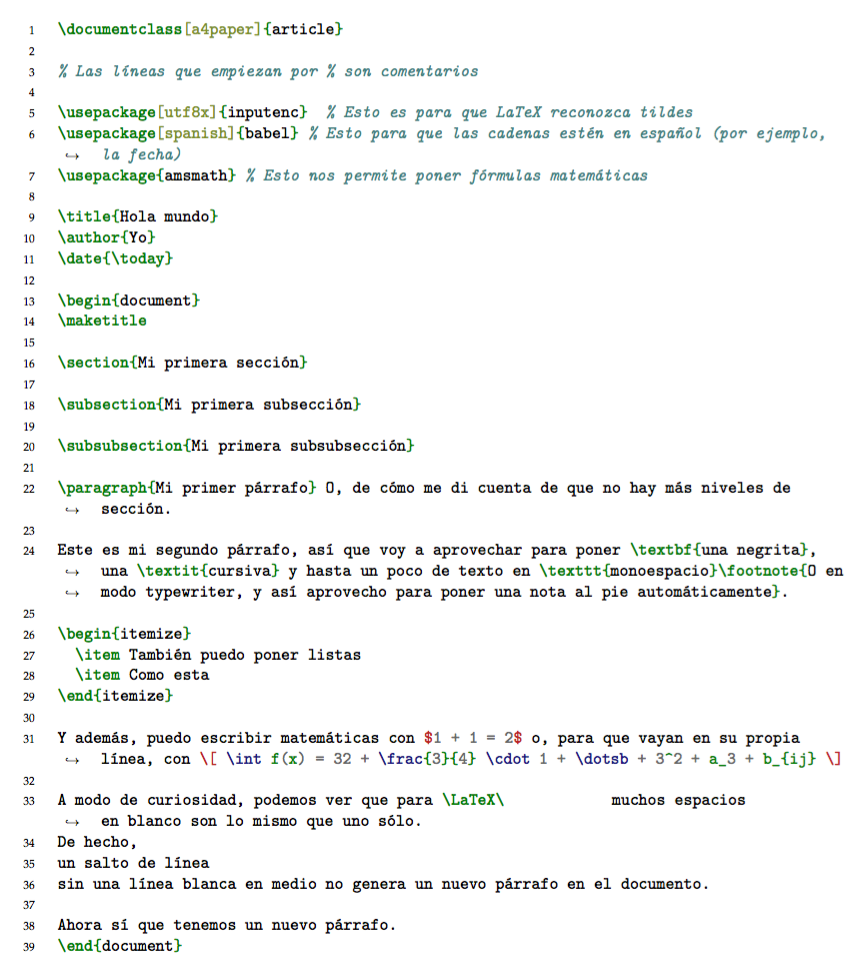
\includegraphics[height = 150pt]{CodigoLatex.png}
\end{minipage}
\begin{minipage}{0.48\textwidth}
\centering
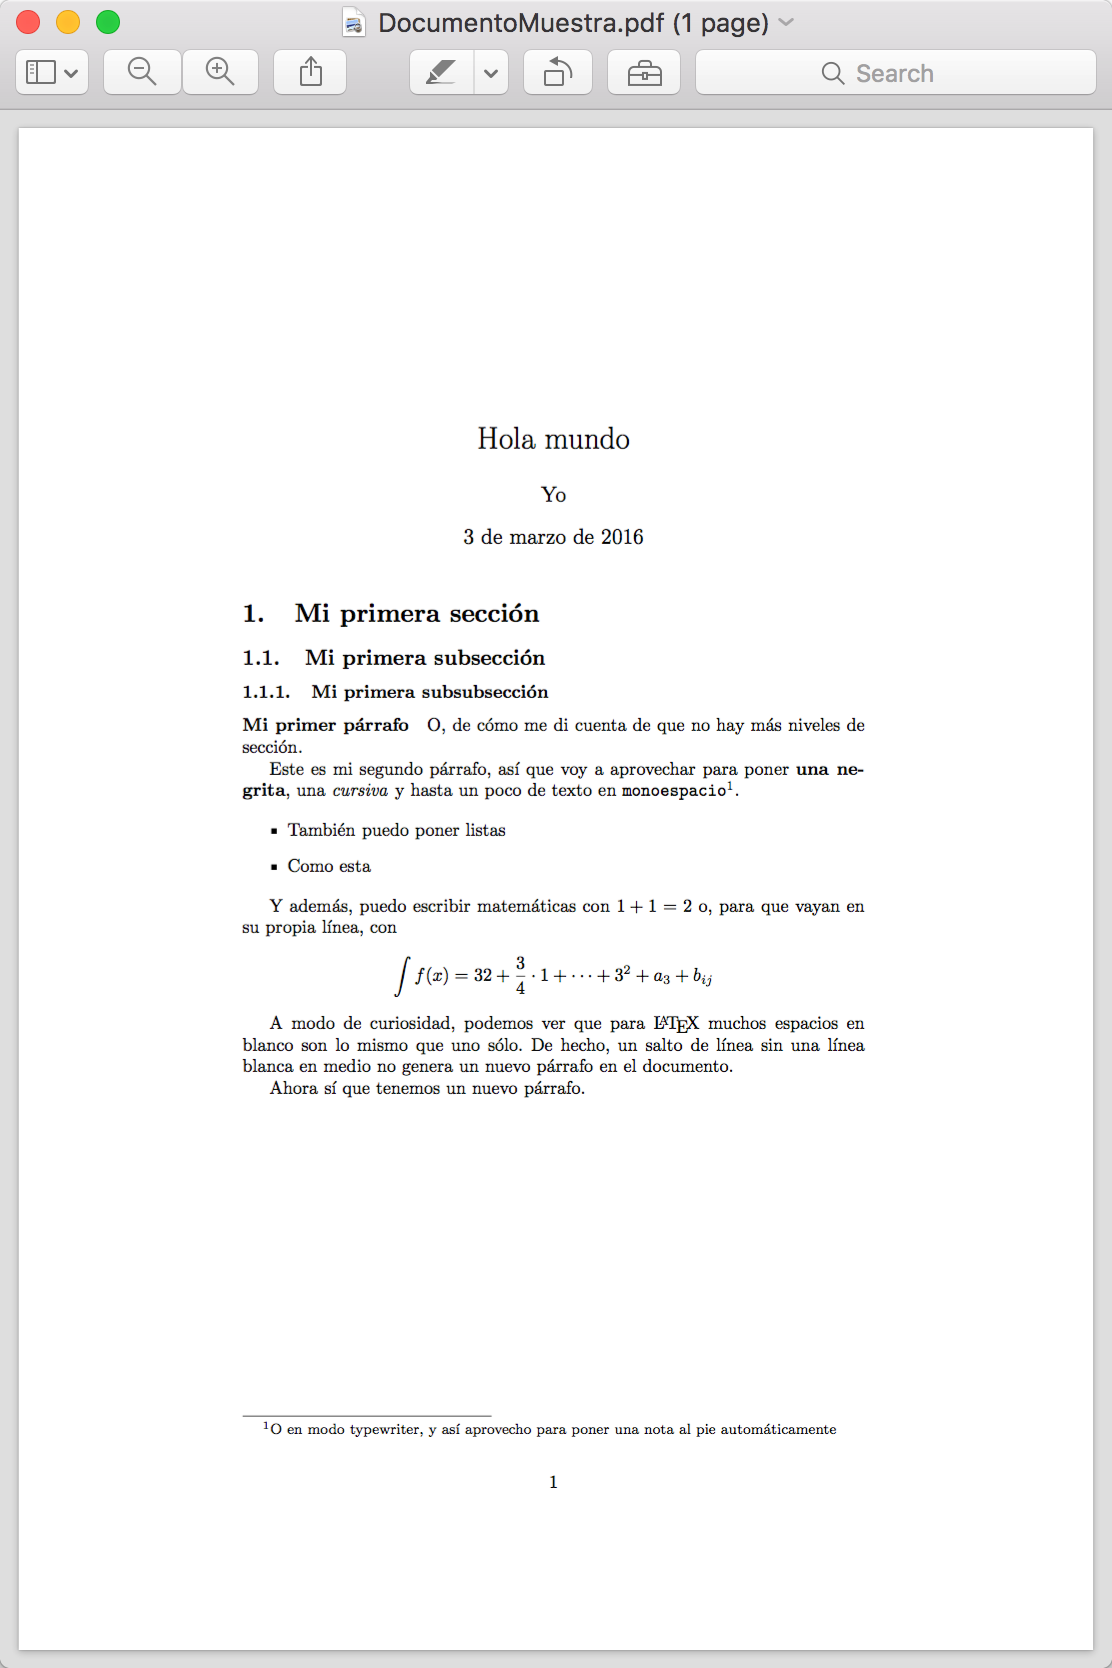
\includegraphics[height = 150pt]{DocumentoFinal.png}
\end{minipage}
\end{figure}

\note{Comentar las ``desventajas'' de usar un compilador: fallos de compilación, tener que hacer varias pasadas para tener todo bien (índice, referencias)... También habría que mencionar \textit{latexmk}, que hace todo esto él solito.

Por supuesto, el compilador tiene ventajas, y la principal es la automatización y la rapidez. Podemos usar el editor que queramos, no hay problemas de compatibilidad...
}

\end{frame}

\end{document}
